\documentclass{article}
\usepackage{graphicx}
\usepackage{svg} 
\usepackage[bottom=4cm]{geometry}

\begin{document}

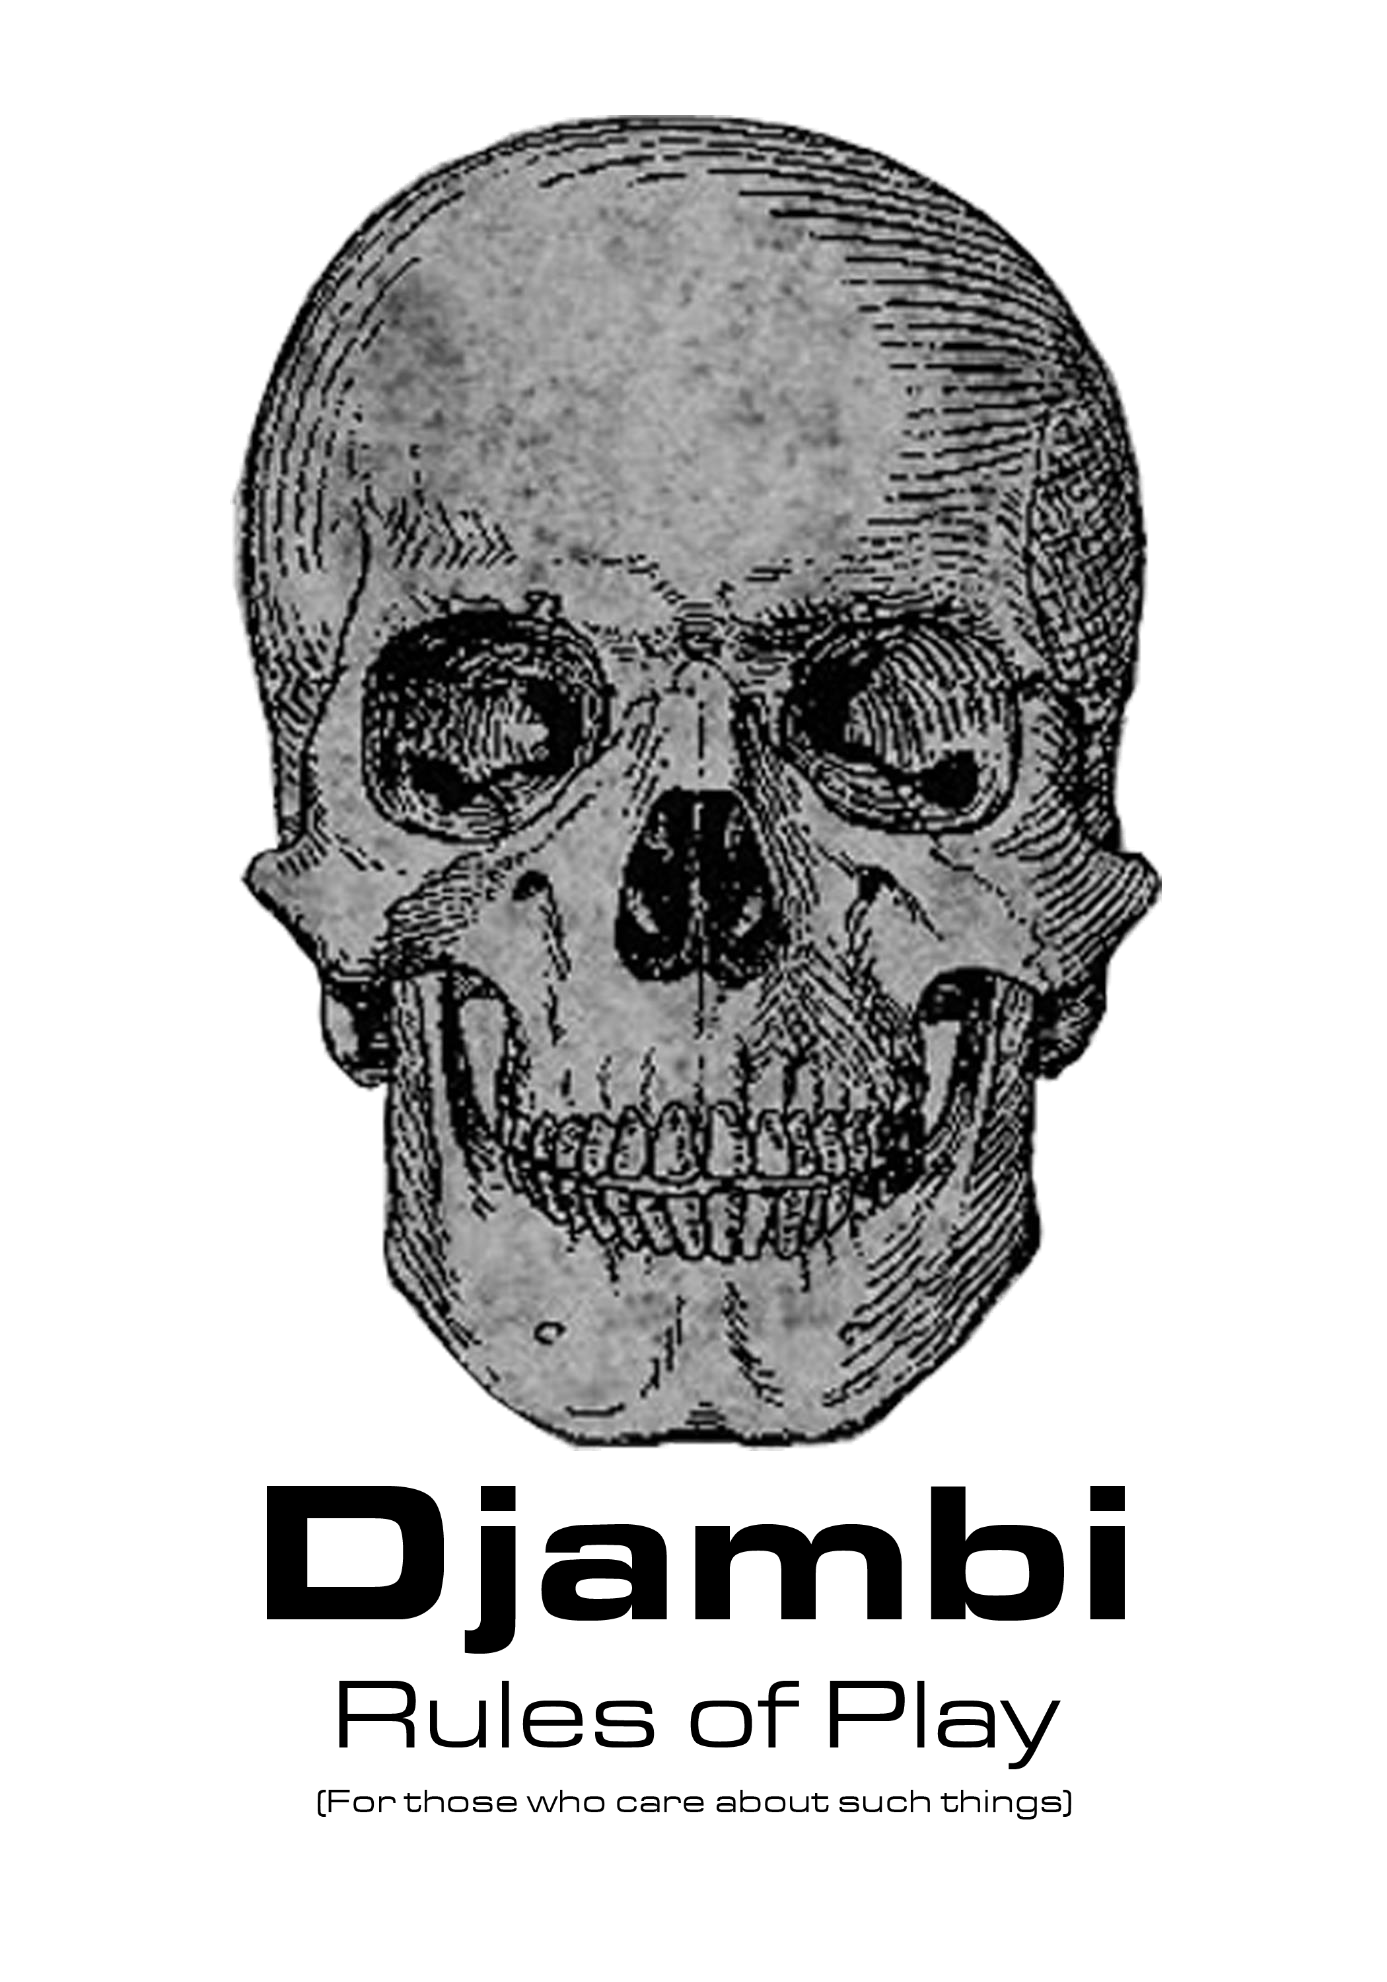
\includegraphics[width=5in,height=7in]{media/image1.png}
\newpage

\tableofcontents

\newpage

\section{Overview}

Au niveau de l'algorithme, on pense à plusieurs stratégies en s'inspirant des échecs.

\subsection{Minimax}

Minimax est l'algorithme classique pour les jeux à deux joueurs. Il est basé sur la recherche d'arbre de jeu.
Il a pour avantage de ne pas avoir besoin d'entraînement. On appelle ça une heuristique.

Le concept est d'évaluer une situation en examinanant les coups et réponses possibles et en évaluant la nouvelle situation à chaque issue.
On s'appuie sur des branches et des feuilles dans cette heuristique. Une feuille est "l'état d'un plateau" en tant qu'instance d'objet.

Quelques challenges à relever avec le djambi: 
- c'est un jeu à plus de 2 joueurs, avec des éliminations possibles
- il y a beaucoup d'états du jeu possibles
- il y a beaucoup de coup possible à chaque tour
- il y a parfois plusieurs actions à faire (choisir où se déplacer, choisir ou placer la pièce tuée..)
- il faut prendre en compte le moment où un joueur prend le pouvoir et peut jouer plus souvent.



\subsection{Reinforcement}

DeepZero a été entraîné avec un algorithme de renforcement. C'est une approche plus moderne et plus puissante que Minimax.
Il est basé sur l'apprentissage profond et l'entraînement sur des millions de parties.
Appliqué au Djambi, il faudrait entraîner un modèle sur des parties de Djambi pour qu'il apprenne à jouer.



\newpage



\section{Règles classiques}
La version historique du jeu est conçue par Jean Anesto en 1975.
Elle se déroule sur un plateau carré avec 4 joueurs.


\end{document}
